%%
%% Copyright 2007, 2008, 2009 Elsevier Ltd
%%
%% This file is part of the 'Elsarticle Bundle'.
%% ---------------------------------------------
%%
%% It may be distributed under the conditions of the LaTeX Project Public
%% License, either version 1.2 of this license or (at your option) any
%% later version.  The latest version of this license is in
%%    http://www.latex-project.org/lppl.txt
%% and version 1.2 or later is part of all distributions of LaTeX
%% version 1999/12/01 or later.
%%
%% The list of all files belonging to the 'Elsarticle Bundle' is
%% given in the file `manifest.txt'.
%%

%% Template article for Elsevier's document class `elsarticle'
%% with numbered style bibliographic references
%% SP 2008/03/01
%%
%%
%%
%% $Id: elsarticle-template-num.tex 4 2009-10-24 08:22:58Z rishi $
%%
%%
\documentclass[10pt,conference,letterpaper]{IEEEtran}
\usepackage{times,amsmath,epsfig}

%% Use the option review to obtain double line spacing
%% \documentclass[preprint,review,12pt]{elsarticle}

%% Use the options 1p,twocolumn; 3p; 3p,twocolumn; 5p; or 5p,twocolumn
%% for a journal layout:
%% \documentclass[final,1p,times]{elsarticle}
%% \documentclass[final,1p,times,twocolumn]{elsarticle}
%% \documentclass[final,3p,times]{elsarticle}
%% \documentclass[final,3p,times,twocolumn]{elsarticle}
%% \documentclass[final,5p,times]{elsarticle}
%% \documentclass[final,5p,times,twocolumn]{elsarticle}

%% if you use PostScript figures in your article
%% use the graphics package for simple commands
%% \usepackage{graphics}
%% or use the graphicx package for more complicated commands
%% \usepackage{graphicx}
%% or use the epsfig package if you prefer to use the old commands
%% \usepackage{epsfig}
\usepackage{todonotes}
%% The amssymb package provides various useful mathematical symbols
\usepackage{amssymb}
%% The amsthm package provides extended theorem environments
%% \usepackage{amsthm}

\usepackage{multirow}

\usepackage{array}

\usepackage{tikz}
\usepackage{pgfplots}

\newcolumntype{L}[1]{>{\raggedright\let\newline\\\arraybackslash\hspace{0pt}}m{#1}}
\newcolumntype{C}[1]{>{\centering\let\newline\\\arraybackslash\hspace{0pt}}m{#1}}
\newcolumntype{R}[1]{>{\raggedleft\let\newline\\\arraybackslash\hspace{0pt}}m{#1}}

%% The lineno packages adds line numbers. Start line numbering with
%% \begin{linenumbers}, end it with \end{linenumbers}. Or switch it on
%% for the whole article with \linenumbers after \end{frontmatter}.
%% \usepackage{lineno}

%% natbib.sty is loaded by default. However, natbib options can be
%% provided with \biboptions{...} command. Following options are
%% valid:

%%   round  -  round parentheses are used (default)
%%   square -  square brackets are used   [option]
%%   curly  -  curly braces are used      {option}
%%   angle  -  angle brackets are used    <option>
%%   semicolon  -  multiple citations separated by semi-colon
%%   colon  - same as semicolon, an earlier confusion
%%   comma  -  separated by comma
%%   numbers-  selects numerical citations
%%   super  -  numerical citations as superscripts
%%   sort   -  sorts multiple citations according to order in ref. list
%%   sort&compress   -  like sort, but also compresses numerical citations
%%   compress - compresses without sorting
%%
%% \biboptions{comma,round}

% \biboptions{}

\title{CAP in practice: HBase and MongoDB}

%% use optional labels to link authors explicitly to addresses:
%% \author[label1,label2]{<author name>}
%% \address[label1]{<address>}
%% \address[label2]{<address>}

\author{Thomas Uyttendaele (thomas.uyttendaele@student.kuleuven.be) \\ 
Departement Computerwetenschappen, KULeuven, Belgi\"e}

\begin{document}

\maketitle

\begin{abstract}
This papers introduces a new, quantified method to test distributed database system in regard to their behaviour to availability in case of a failing node and consistency of data from the users perspective. This method is tested on HBase and MongoDB, two consistent and partition tolerant systems, some interesting outcomes are described in this paper. 
\end{abstract}

%%
%% Start line numbering here if you want
%%
% \linenumbers

%% main text
\section{Introduction}

New online services and more online users means more data, data and load a single server can't handle. Database systems are transformed towards a more distributed approach, for higher availability in case of an unexpected crash but also for horizontal scalability: the data of a single database is spread over different systems. Several new software have other requirements on the database than a few years ago; e.g. a change in a record doesn't need to be read correctly by other users immediately, this can happen in time. This behaviour is called eventual consistency. 

Over the past years, many new systems have been build on this wave of changes, categorized as NoSQL. Some applications contain a high volume of data, have the need for consistent data and need to work in a highly distributed environment, this are the CP systems in the CAP Theorem. Two examples that offer these guarantees are HBase and MongoDB. They greatly differ in supported queries on their system. But what happens if you only use the bare essentials and compare their behaviour in a distributed environment going from expected shut downs of instances towards crashes and network partitions? 

In this article, a comparison of this systems will be described. In chapter \ref{sec:CAPTheorem} a brief overview of the CAP Theorem is given, chapter \ref{sec:hbaseandmongodb} discusses HBase and MongoDB based on the literature. Chapter \ref{sec:testmethod} gives an overview of the used test method and chapter \ref{sec:result} presents the results. The future work is presented in chapter \ref{sec:futurework}, an overview of related work is given in chapter \ref{sec:related work} and a conclusion is formulated in chapter \ref{sec:conclusion}.  

\section{The CAP Theorem\cite{brewer2000towards}\cite{brewer2012cap}}\label{sec:CAPTheorem}
The CAP Theorem was introduced by E. Brewer \cite{brewer2000towards}  in 2000 and discusses three properties of which each network shared-data system can guarantee at most two: (definitions based on \cite{brewer2012cap})
\begin{itemize}
\item (Strict)\textbf{C}onsistency: The system acts like there is only single storage 
\item High \textbf{a}vailability: The system is available (for updates)
\item \textbf{P}artition tolerance: A split in the network let the different partitions still act as a single system. 
\end{itemize}
Designers used this model to explain their design decisions, others used it to compare different system and sometimes it was misused. As E. Brewer explains 12 year after the launch, the "2 of 3" can be misleading.

One of the reasons is that there exist several types of consistency, partition tolerance and there are different availability guarantees. The choice for the properties needs to be made several times in the different subsystems and the end solution is not black or white. 

At first glance, it also looks like partition tolerance has to be implemented and therefore consistency or availability needs to be given up. In the practice, partition splits are only rare and therefore both consistency and availability can be allowed most of the time. 

Each of the 3 choices will be discussed in more detail, how their implementation could work, what the influences are and some examples. 

\subsection{CA: Consistency and availability}
When forfeiting partition tolerance, these systems provide all the time consistent data available to all nodes, except when there are one or more nodes unavailable. In that case, write requests will be not allowed. 

These systems can be build based on the two phase commit and have cache invalidation protocols. Examples of this types are the typical relational databases roll out in clusters. 

\subsection{CP: Consistency and partition tolerance}
A consistent system with partition tolerance will provide all the time the last data, even in the case of network splits. This comes with the loss of the availability of some nodes during the partition time.

The system can allow operations only on the majority partition. In case multiple splits are present and no partition has a majority of nodes, the whole system can be unavailable. These systems can be build around a master/slave principle where the operations will be directed to the master, the slaves are present to continue operation when the master fails.

In practice, systems like MongoDB, HBase and Redis select CP. 

\subsection{AP: Availability and partition tolerance}
In a highly available systems with partition tolerance. It is possible to read inconsistent data. As read and write operations are still allowed when there are different partitions, it is possible that the database has other content depending on the used node. When the split is dissolved, a need for manual conflict resolution can be needed. In case a record is adapted in both partitions, the user will need to choose the correct version. 

Example systems following AP are Cassandra, Riak and Voldemort. 

\section{Overview of HBase and MongoDB}\label{sec:hbaseandmongodb}
In this article, 2 CP systems will be discussed more in detail regarding their choices to forfeit availability and the influence on their behaviour in practice. The systems are HBase and MongoDB, an architectural overview will be given in this section. 

\subsection{HBase}
HBase\cite{hbase-doc} is an open-sourced, distributed, versioned database designed after Google's BigTable \cite{chang2008bigtable}. HBase relies on Zookeeper for the distributed task coordination. The persistent storage can be done on the local hard disk, Hadoop Distributed File System or Amazon S3. In this article is chosen for Hadoop. 

HBase nodes exists out of HMasters and HRegionServers, the coordination of the system is done by one HMaster, the handling of data is done by the HRegionServer. Multiple Hadoop datanode instance should be deployed for data storage, preferable one on each HRegionServer. The data will be replicated to a configurable amount of other nodes, default modus is 3. The data is stored in a table, which is split in one or more regions. A region is leased to a given HRegionServer for a defined time. During this time, only this server will provide the data of the region to the different users. This way the consistency of data is guaranteed due to the fact that there is a single system responsible for the storage of a record.  Consistency on a single record is provided by a readers/writer lock on a single record for the according queries, this way there is a guarantee to atomicity on a single record, the full procedure is explained by Lars Hofhansl\cite{hbase-acid}. 

To be partition tolerant, the partition with the majority of the Zookeeper servers and a HMaster will appoint regions to available HRegionServers, let's call this the data serving partition. In this approach, it is important to place the Zookeeper and HMaster servers in diverse location as otherwise a partition of only management servers will make the whole system unavailable. 

In HBase, a node will be able to reply to requests if the node is present in the data serving partition. Only in rare cases that all data copies of Hadoop are stored in unavailable servers, the data will be unreachable. The nodes that are not in the data serving partition, will be unable to complete any requests. 

When a server goes down, he can release the lease in case there is a graceful shut down (the HBase server is notified) and another server can get the lease immediately. In other cases, a new lease can only be given after the decay of the old lease, if the server comes back online in meantime, he will still be responsible. 

\subsection{MongoDB}
MongoDB\cite{mongodb-doc} is an open-sourced, distributed database designed for document storage, this are data entries where the format of each record can be different. According to their website they provide high performance and high availability, but this is incorrect to the given definition in this article. 

MongoDB provides data replication and data distribution. The first is done by grouping different MongoDB servers into a ReplicaSet. The second is done by grouping different of these ReplicaSets and dividing the data between them.  

A ReplicaSet exists out of different MongoDB servers whom work as master and slaves. A master is a primary and a slave is called a secondary. The primary is responsible for the write actions, by default a query will succeed once it has a confirmation that the write has been executed on the primary. The read operation will go by default on the primary as well. Both query methods are configurable to give other guarantees. For a write operation there are multiple \textit{write concerns}, it is possible to wait till it has written on hard disc or a number of secondary servers, however all need a primary. For read operation there are multiple \textit{read preferences}, it is possible to read from a secondary or the closest server. \\ 
In the default configuration, MongoDB provides a consistency guarantee.

In a ReplicaSet, there is at least half of the ReplicaSet needed for the primary election. As there is always a primary needed, the system has partition tolerance but no high availability, contrary to the statement on the documentation. However, it is possible to read from a secondary but writing is not possible.

The liveness of the different members of a ReplicaSet is maintained by a heartbeat system: a server is marked as offline if no beat has been received for 10 seconds. In case the primary goes offline, election will be started to re-elect a new one. In other words, a primary has a lease of 10 seconds. This value of 10 seconds is non-configurable. 

De data distributions happens by merging replica sets in a cluster. Furthermore, there is the need for access server (as many as you want) and configuration servers (1 or 3). The availability and partition tolerance of the data is the same as in the ReplicaSets as it handled by the ReplicaSets. In case a access server can't reach a primary, another access server will be needed to write data. If a majority of the configuration servers are not reachable, their will be no reconfiguration of the data over the different servers.  

\subsection{Differences between databases} 
Both systems provide consistency and partition tolerance and forfeit high availability, but some differences are in their implementation. 

First of all, they differ in their handling of partition tolerance. HBase has dedicated management servers (HMaster and Zookeeper) to distribute the responsibilities of regions and if the management servers are in a partition with a minority of the data servers, data will be not available. In MongoDB the management of a ReplicaSet is done internally with as result that the write queries will be available in the partition with the majority of the data servers.

Both decisions have their reasons and possible motivations, in HBase it is possible to write every record, as a new region can be created if the old region is unavailable. In MongoDB it is possible that in sharding you can read all the data from multiple secondaries but only write given ranges of records.

In availability, there is a small difference: where in MongoDB it is possible to read from secondaries, this is impossible in HBase. 

In section \ref{sec:result}, a detailed analyse will be done to the consistency and the behaviour of the systems in the case of network or server failure. 

\section{Test method}\label{sec:testmethod}
To test the behaviour of database systems towards consistency and availability, the Yahoo Cloud Serving Benchmarking (YCSB \cite{cooper2010benchmarking}) has been extended with event support for availability and reader-writer support for consistency.

Each of this tests follows the same steps: calibrating the system, records are preloaded, the test is started and in the end all the records are removed again and they are executed for HBase and MongoDB. During the calibration, a workload is chosen so there is a medium load on the different databases. 

\subsection{Event support}
The implementation of event support is integrated in YCSB so it supports the execution of UNIX commandos at specified moments. The execution time and result code is logged. 

Before the test are 300 000 records stored in the database to enable the sharding in all database softwares. These tests contains 3 kinds of tests, of which an individual test takes 900 second. The first action takes place at 300 seconds, the second at 600 seconds.
\begin{itemize}
\item (1) Graceful shut down of a data service and (2) restart of the service
\item (1) Hard kill of the data service and (2) a restart of the service
\item (1) Blocking of all network traffic from and to a server and (2) the allowance of all network traffic
\end{itemize}

Each element tests the behaviour of the system under different circumstances, the first two checks what happens in case of a respectively planned and unexpected shut down, the latter check the behaviour in case the network fails or a server crashes.

The tests are executed on each of the data nodes of HBase and MongoDB.Caching and buffering on the client side are disabled in both tests. 

\subsection{Consistency support}
To implement consistency support, the YCSB software is extended with an extra workload. A graphical representation of an example workload is shown in figure \ref{fig:consistence-method}. 
\begin{figure}[ht]
\centering
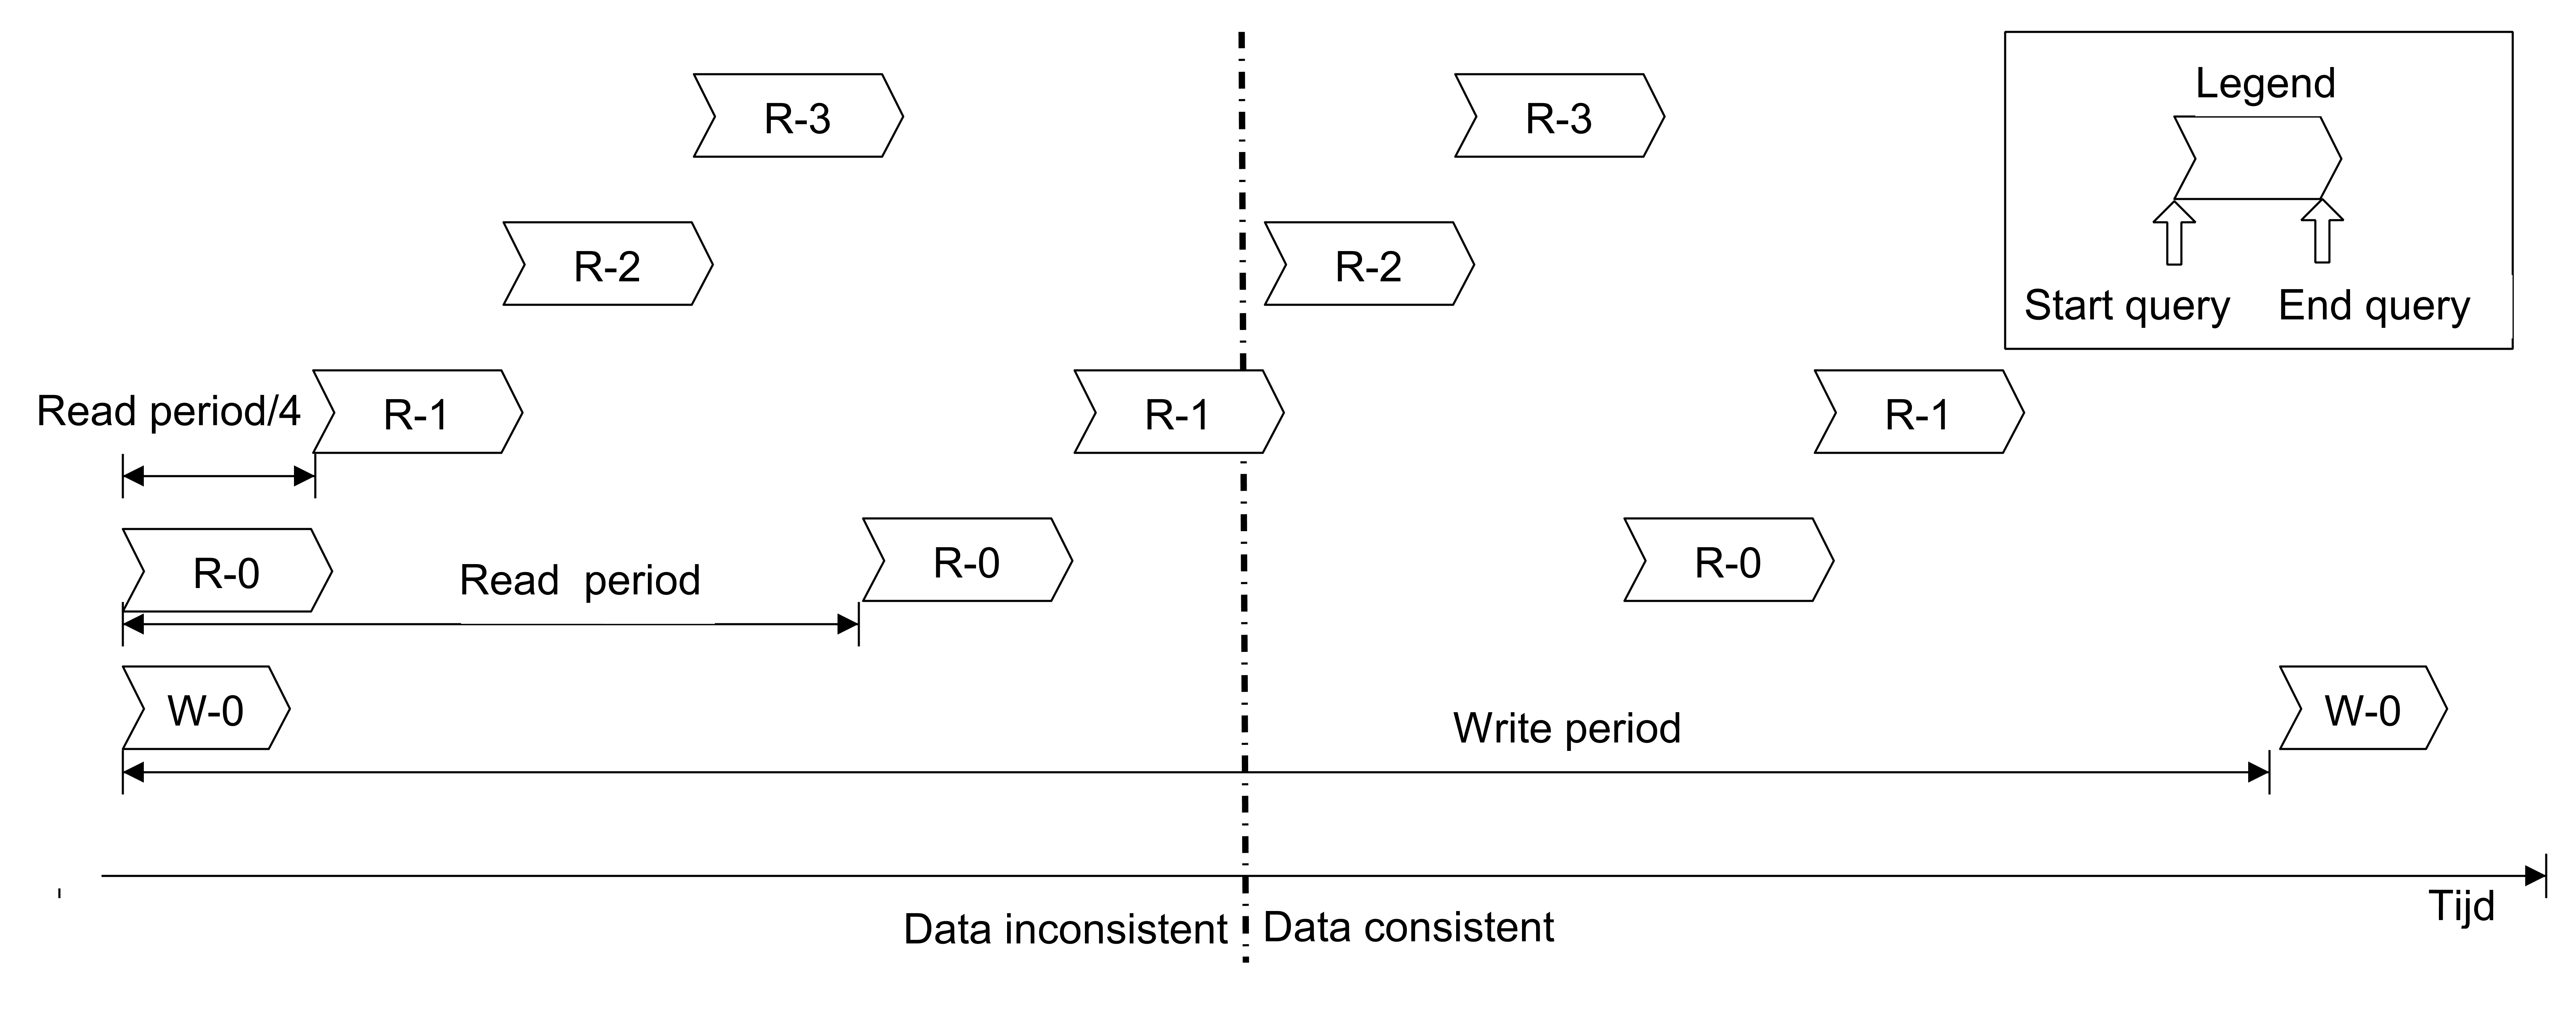
\includegraphics[width=\linewidth]{../img/Consistency-test-period}
\caption{Example of consistency support for one write period with 1 writer and 4 readers}
\label{fig:consistence-method}
\end{figure}
This workload exists out of 1 writer and a user-defined amount of readers.  Each writer will insert or update a value in the database at a user-configurable pace. The readers will read the record till they read the last written data element, each reader reads in a period defined by the user. The different readers are scheduled uniformly within the reading period. 

All this data is logged and gives possibilities to analyse when a record is visible for different users, compared to the time when the queries were started or ended. 

Before the test, there are 30 000 records stored in the database, each tests takes 500 seconds and results start to be gathered after 30 seconds. In the tests is chosen to write every 0.5s and read with 5 readers every 10ms in MongoDB. In HBase there are 10 readers who read every 30ms.  
 

\section{Results}\label{sec:result}
To execute the tests, both systems were deployed on a virtual platform of OpenStack. Each instance has 2 CPUs, 4GB RAM and 50GB disc space. The machines are connected with a gigabit Ethernet and an average ping takes 0.4ms ($\sigma = 0.2$ on 10 000 ping's).

HBase is configured with 5 instances, of which 1 for management (HMaster, Hadoop namenode and Zookeeper) and 4 for data storage (each has a HRegionServer and Hadoop datanode). 

MongoDB is configured with 6 instance, grouped by 3 in a ReplicaSet. There was a single configuration server and 3 instances had an access server. 

YCSB was deployed on a single instance and used to calibrate the load on both systems. An individual record has 10 fields which each field a size of 100 bytes. The workload existed out of 20\% inserts and updates, 40\% selects and 20\% scans of an uniform spread between 1 and 100. The order of the reading and updating of the records is defined by a Zipfian\footnote{Some record are popular, others rare to be used.} distribution. The basic load for HBase is an average of 600 queries/second spread over 50 threads, for MongoDB there are 15 threads with a total of 200 queries/second. 

\subsection{Availability}
When reading and writing in the default setting of MongoDB, both MongoDB and HBase will read and write from a leader of a set of data. Both have a lease period for the leader, which can't be set for MongoDB (10 seconds), but can be configured for HBase (default 180 seconds). 

\begin{figure}[ht]
\centering
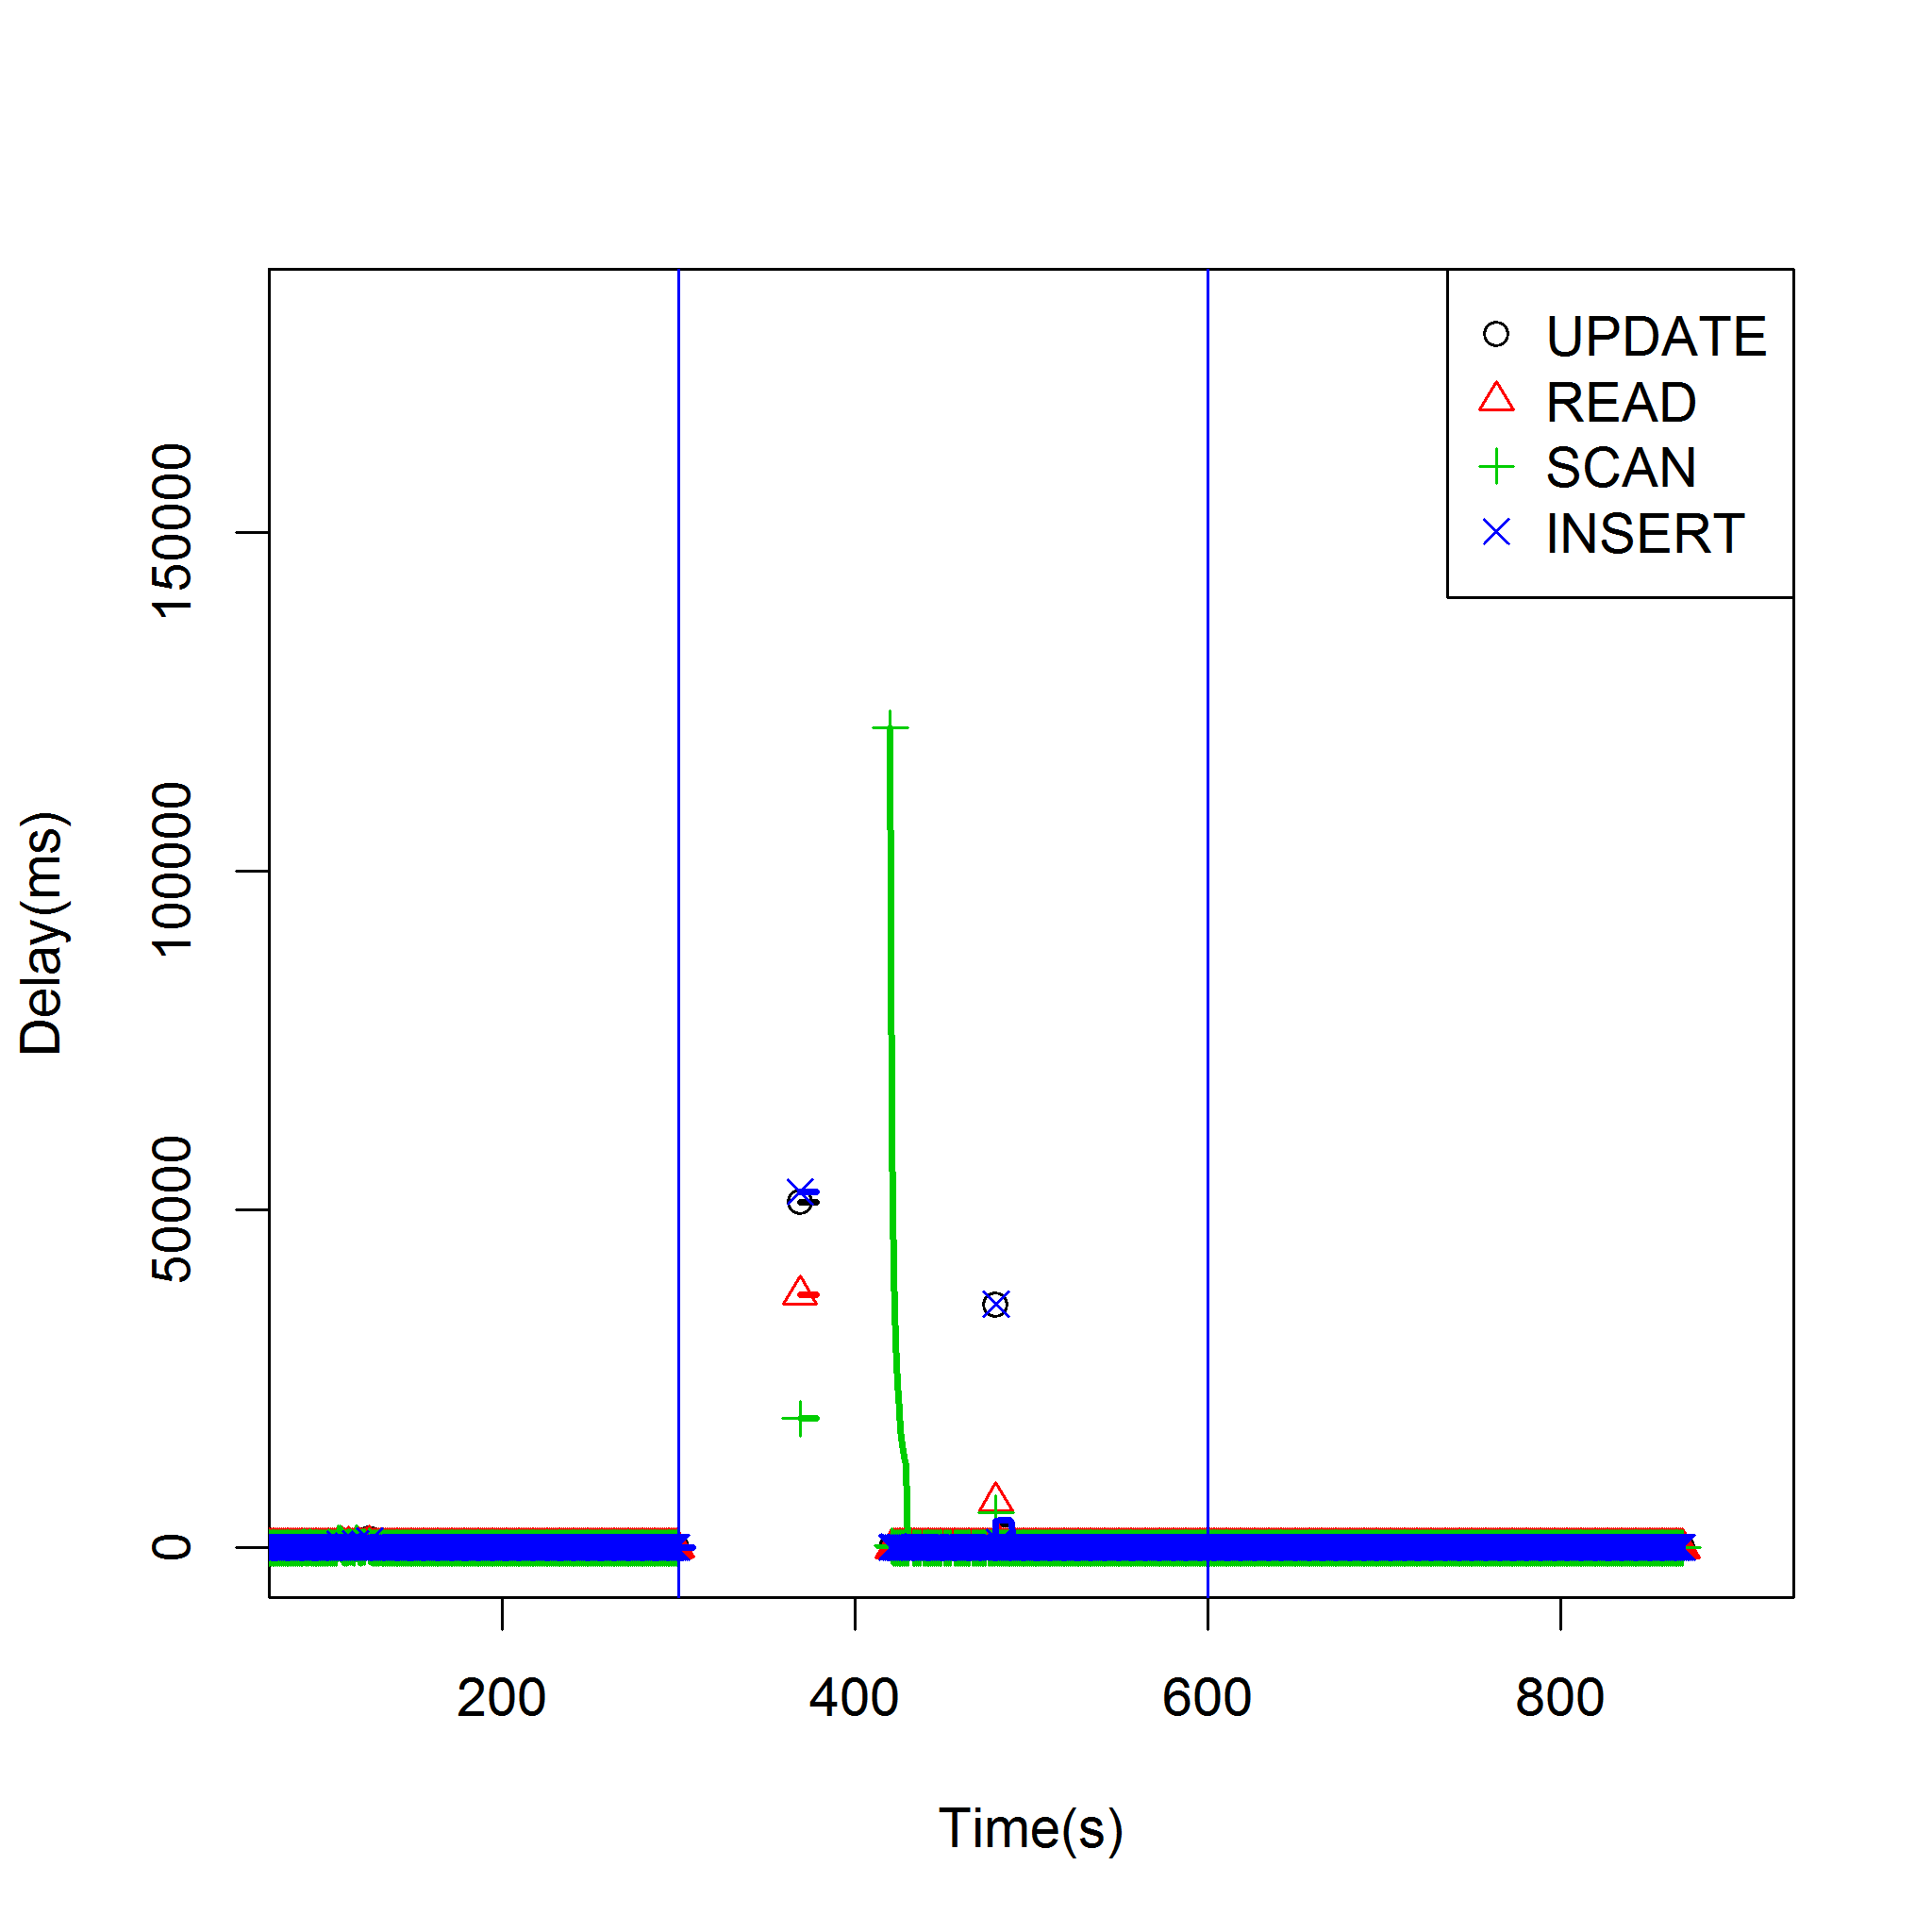
\includegraphics[width=\linewidth]{img/HBase/single-graph-2-drop-1}
\caption{Example of network partition. The requests block for 110 seconds }
\end{figure}

In case of a stop of a HBase server in this configuration, the queries will halt till the lease for the region has been expired, this can take between 0 seconds and 180, depending on the moment of the action. In case of a graceful stop of the service, the service will release the lease and a faster handover is possible. During the tests it happened that with a hard stop of the service, no queries can be executed on the database connection till the server is brought back online. In this scenario it was needed to manually dis- en reconnect to the database. A reason why this happens is still unknown.

For MongoDB, there is no difference between the graceful or hard stop of an instance; in case it was a secondary, no influences on the latency will be seen. In case a primary was stopped, the data will be temporarily unavailable for a few seconds. It seems that in a hard stop, there is still a messaging of the shut down to the other nodes. In case of a network interruption, the results are varied. It goes from no influence, a temporary unavailability for a few seconds, or no completed queries the whole time the server is down. If all connections are reinitialised for the last case, new queries can executed. If this is not done the table seems empty. 

A short overview of all the reactions is shown in table \ref{table:beschikbaarheid-stop-resultaat}. 
\begin{table}[htbp]
  \centering
  	\scalebox{0.8}{
      \begin{tabular}{l | lll}
          & Graceful stop & Hard stop & Network partition\\
    \hline
    \multirow{2}{*}{HBase} & Few seconds & Dozens of seconds & Dozens of seconds \\
    & & to unlimited&  \\
    \multirow{2}{*}{MongoDB} & 1/3 of the cases, & 1/3 of the cases, & Few seconds to  \\
    & Few seconds & Few seconds & unlimited\\
    \end{tabular}%
    }
    \caption{Availability: Overview of different reaction when stopping an instance }
  \label{table:beschikbaarheid-stop-resultaat}%
\end{table}

\subsection{Consistency}
Based on consistency, HBase and MongoDB have a different approach. In MongoDB it is possible to configure the read and write queries, in HBase there is the choice to use cache at client side. In the tests the cache is disabled but the different options of MongoDB are tested. 

HBase: If a record is read while a write query is inserting or updating the value, the read query will wait till the completion of the write query and return immediately the correct value. If a read query is send too soon, it will return the old data. Each query that is finished after the completion of a write query, will return the new data. A graphical representation of this can be seen in figure \ref{fig:consistentie-hbase-voorbeeld}. The stop time of the reader follows the one of the writer, together with extra information, it can be concluded that this is coming from the blocking till the write query has finished. 

\begin{figure}[h]
\centering
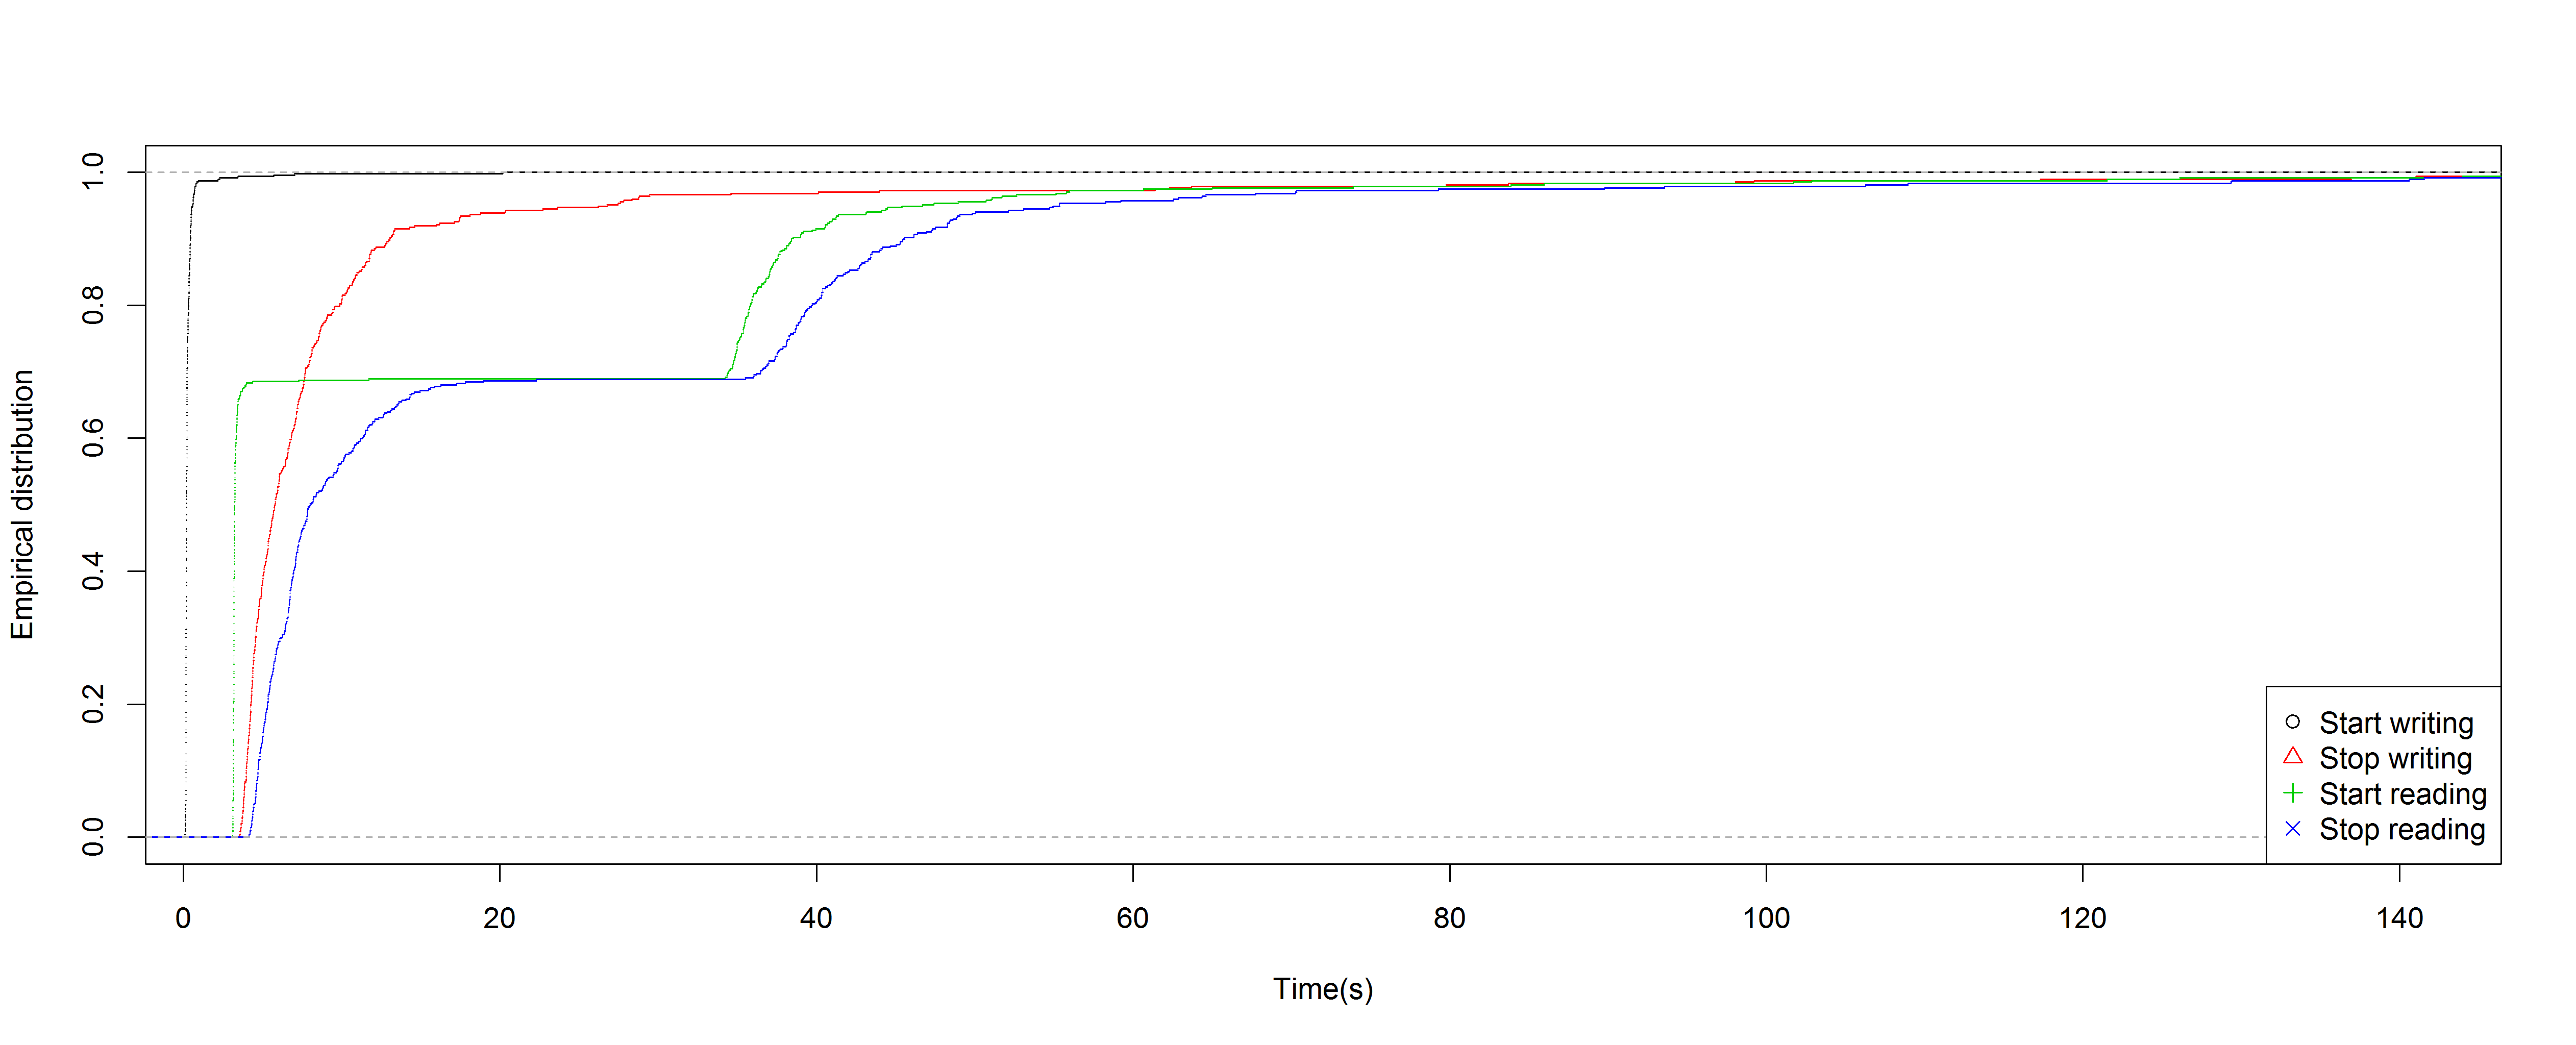
\includegraphics[width=\linewidth]{img/HBase/ECDF-plot-R-1-insertRawData-5}
\caption{Consistency: cumulative distribution of queries that read the correct value if reading is started 3ms, 13ms, 23ms. Measurement of over 400 values.}
\label{fig:consistentie-hbase-voorbeeld}
\end{figure}

MongoDB: A read query can return the old or new data before the write query has been completed. Despite of the use of a readers/writer lock mechanism, it seems that after releasing the lock, the write query still has to execute extra steps. When reading from a secondary or the nearest server, there will be monotone read consistency, except if the driver of MongoDB selects another server between the reads, as there is no guarantee that the other servers already have the value. The process of finding the nearest server happens periodically in the background. \\
From the test results, the writer configuration has no influence on consistency window for the different readers if the start moments of the writers and the successful read queries are compared. The difference is the guarantee a user has when a write query has finished. 

An overview of the consistency windows is shown in figure \ref{fig:consistentie-hbase-correct} and \ref{fig:consistentie-mongodb-correct} for respectively HBase and MongoDB. 

\begin{figure}[!htf]

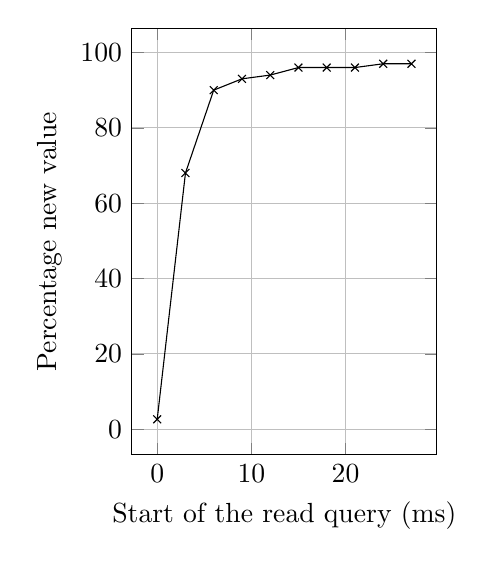
\begin{tikzpicture}
	
	\begin{axis}[
		xlabel={Start of the read query (ms)},
		ylabel={Percentage new value},
		domain = 0:1,
		grid = major,
		height=7cm,
		width=.45\textwidth
	]
	

	\addplot[color=black,mark=x]
	        plot coordinates {
	       		(0, 2.6)
				(3, 68)
				(6,90)
				(9,93)
				(12,94)
				(15,96)
				(18,96)
				(21,96)
				(24,97)
				(27,97)
	        };

	\end{axis}
\end{tikzpicture}
\caption{Consistency: Percentage of the queries started at the given time moment that will read the newest inserted data. The average latency in a random read transaction is around 6ms.}
\label{fig:consistentie-hbase-correct}
\end{figure}

\begin{figure}[!htf]

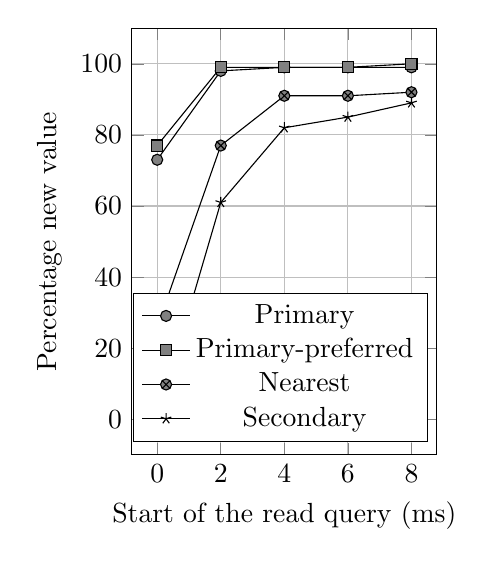
\begin{tikzpicture}
	
	\begin{axis}[
		xlabel={Start of the read query (ms)},
		ylabel={Percentage new value},
		domain = 0:1,
		grid = major,
		height=7cm,
		width=.45\textwidth,
		legend pos= south east,
		cycle list name=black white
	]
	
		\addplot
		        plot coordinates {
		       		(0, 73)
					(2, 98)
					(4,99)
					(6,99)
					(8,99)
		        };
		\addlegendentry{Primary}
		
		\addplot
	      plot coordinates {
		       		(0, 77)
					(2, 99)
					(4,99)
					(6,99)
					(8,100)
	      };
		\addlegendentry{Primary-preferred}
		
	\addplot
	        plot coordinates {
	       		(0, 26)
				(2, 77)
				(4,91)
				(6,91)
				(8,92)
	        };
	\addlegendentry{Nearest}


	
	\addplot
   plot coordinates {
	       		(0, 0)
				(2, 61)
				(4,82)
				(6,85)
				(8,89)
   };
	\addlegendentry{Secondary}
	\end{axis}
\end{tikzpicture}
\caption{Consistency: Percentage of the queries started at 0, 2, 4 and 8ms  that will read the newest inserted data with the each row for MongoDB. The average latency on a read transaction is for all read queries around 1ms. }
\label{fig:consistentie-mongodb-correct}
\end{figure}


\section{Future work}\label{sec:futurework}
The test executed on the different systems are a start to have a quantified approach on the consistency and availability of the different systems. Besides testing more systems, deeper testing can be done and extensions can be added to the benchmarking tool.

First of all, the strange behaviour of MongoDB and HBase of not allowing connections, could be researched in more detailed. 

Secondly, the third element of CAP can be included: Partition tolerance. Right now the connection nodes are chosen when setting up the test, an extension could be to test all connections and see what happens in the case of a partition tolerance. How is the availability of each node? How long is a primary in MongoDB still accepting queries after it has been cut off from the other instances? 

Thirdly, the availability and consistency tests could be tested together: when a node is shut down or cut off, is there the loose of data? Especially in MongoDB it could be the case that the data is already read on the primary but not yet replicated to the primary, what happens if the primary is cut off? 

At last, the test parameters could be adapted, what happens with a different network infrastructure when the network distance is not equal any more, what happens with a higher and lower load? It could be possible to come up with a mathematical formula which could predict the average consistency window for example.  


\section{Related work}\label{sec:related work}
The is only a limited amount of research executed towards the guaranties a database system provides towards consistency and availability. In recent paper (February 2014), Golab et al. states that there is only a limited amount of research done towards eventual consistency \cite{golab2014eventually}. They present the current research and describe a missing category of testing methods towards consistency. This category is called the passive analysis, this analysis focusses on how a database user observers the consistency guaranties. This is different from the active analysis where they mostly focus on the time it takes to replicated to all nodes.  With the testing method described in this paper, both are covered: as well the delays before the data is present everywhere but also on the acting of the specific systems, in example the behaviour of HBase. 

Another extension of YCSB called YCSB++\cite{patil2011ycsb++}, provides more logging information on all systems in the first place, but they also test the consistency of HBase in regards of the client caches. These caches are by default enabled on the client side, but the submission of the client cache towards the system does not only depend on the time. Also the amount of traffic generated at the client influences this speed. In the study they compare different cache sizes and this shows already a difference in time. In case data needs to be strict consistent, it is better to disable caching at this moment, this way the behaviour is more predictable and in general also faster available for other clients. 

For availability benchmarking, there was no research found on related databases. However, research from 2004 \cite{mauro2004system} discuss a way to let a standalone system recover and provide a starting benchmark for it.  


\section{Conclusion}\label{sec:conclusion}
A new testing method to quantify consistency and availability has been presented in this paper. With this method the effect of a stop of an instance can be measured and also the consistency window for different readers. 

Another contribution are the results for two consistent and partition tolerant systems, HBase and MongoDB. These 2 systems are tested with the new method and show their relevance. According to the documentation, MongoDB and HBase both guarantee strict consistency but based on our results their characteristics are different: HBase blocks read queries till the completion of the write queries to guarantee a read will always be the same, MongoDB returns the ready query soon with new or old data before the write operation has been finished. 

In the availability of the systems, HBase is in the standard configuration longer unavailable but with a change in the session time out, they can be made more the same. In some occasions both systems have a strange behaviour of not returning any results, in the case of HBase this is for a hard stop, in the case of MongoDB it is for a network partition. This doesn't happen in the other situations and in case of reconnecting to the database, the problems are solved. 
%% The Appendices part is started with the command \appendix;
%% appendix sections are then done as normal sections
%% \appendix

%% \section{}
%% \label{}

%% References
%%
%% Following citation commands can be used in the body text:
%% Usage of \cite is as follows:
%%   \cite{key}         ==>>  [#]
%%   \cite[chap. 2]{key} ==>> [#, chap. 2]
%%

%% References with bibTeX database:

\bibliographystyle{elsarticle-num}
\bibliography{referenties}
%% Authors are advised to submit their bibtex database files. They are
%% requested to list a bibtex style file in the manuscript if they do
%% not want to use elsarticle-num.bst.

%% References without bibTeX database:

% \begin{thebibliography}{00}

%% \bibitem must have the following form:
%%   \bibitem{key}...
%%

% \bibitem{}

% \end{thebibliography}


\end{document}

%%
%% End of file `elsarticle-template-num.tex'.
